\maketitlesupplementary

\Crefrange{sec:s:optics}{sec:s:evaluation} specify the optical model, training, reconstruction and evaluation. Full results, structural tests and acquisition controls follow in \cref{sec:s:results,sec:s:structure,sec:s:budgets}; \cref{sec:s:uncertainty,sec:s:views} give complementary uncertainty analyses and neuronal display conventions. Section, equation and figure numbers without an S prefix refer to the main paper. Unless stated otherwise, additional experiments use the 12 prespecified neuronal crops, with five direction subsets at $C>1$. \Cref{tab:s:evidence} summarizes the evaluation units and controls.

\begin{table*}[t]
\centering\small
\begin{tabular}{p{1.55in}p{1.9in}cp{1.95in}}
\toprule
Study & Reference units & Draws & Results \\
\midrule
Five designs, four methods & 60 crops, six cells, three animals & 5 & \Cref{tab:s:e2e,tab:s:criteria60,tab:s:criteria60intervals} \\
Optical sampling seed 1 & Same 60 crops & 5 & \Cref{tab:s:main,tab:s:objectives,tab:s:seedmatched} \\
Phase/amplitude controls & 12 crops, pretrained PnP & 5 & \Cref{tab:s:untrained}; centroid/intensity metrics \\
In-focus DMD & 12 crops, three iterative methods & 5 & \Cref{sec:s:results} \\
Point-emitter diagnostics & 25 positions, 16 depths & -- & \Cref{sec:s:results} \\
Full scan ($C=1$) & 12 prespecified crops & 1 & \Cref{tab:s:compression,tab:s:jointfullscan} \\
Compression, dose, alignment & 12 prespecified crops & 5 & \Cref{tab:s:compression,tab:s:dose,tab:s:alignment} \\
Noise and reduced-dose crops & 12 prespecified crops & 5 & \Cref{tab:s:noise,tab:s:jointdose} \\
Merged-depth alternatives & 59 eligible test crops & 5 & \Cref{fig:s:klalternatives}; \cref{sec:s:structure} \\
Equal-branch crossings & 36 phantoms, including zero gap & 5 & \Cref{tab:s:crossings,tab:s:jointcrossings} \\
Weak/three-filament tests & Cases specified in \cref{sec:s:structure} & 5 & \Cref{tab:s:crossings} \\
Reduced-dose crossings & 24 phantoms, including zero gap & 3 & \Cref{tab:s:jointdose,fig:s:lowdose} \\
Conformal intervals & 35 calibration crops; 12 test crops & -- & \Cref{tab:s:conformal} \\
Reduced-field bounds & 24 phantoms; 48 neuronal windows & 3 & \Cref{sec:s:uncertainty} \\
\bottomrule
\end{tabular}
\caption{Evidence map. Draws are averaged within crops or phantom cases before paired statistics. Crops from the same cell are grouped during the cell bootstrap. The reduced-field row counts noise realizations per phantom. Conformal calibration follows its separate protocol in \cref{sec:s:uncertainty}. Both are complementary analyses.}
\label{tab:s:evidence}
\end{table*}


\section{Optical implementation and discretization}
\label{sec:s:optics}

\paragraph{Coordinates and angular scan.}
The optical axis is $z$ and $\mathbf r=(x,y)$ is transverse position. In the simulated input medium, $n=1$ and $k_{\mathrm{ex}}=2\pi/\lambda_{\mathrm{ex}}$. The incident direction is
\begin{equation}
\mathbf k_t/k_{\mathrm{ex}}=
(\cos\theta_t\cos\alpha_t,\cos\theta_t\sin\alpha_t,\sin\theta_t).
\end{equation}
Thus, $\theta$ is the implemented vertical-plane parameter, not a polar angle from the optical axis. We use $\alpha_m=m\pi/16$, $m=0,\ldots,15$, with eight equally spaced $\theta$ values in each of $[\pi/6,\pi/3]$ and $[2\pi/3,5\pi/6]$. The second interval changes the sign of the transverse component while retaining positive longitudinal propagation. The resulting 256 directions are distinct. For $C=4$ and $8$, five fixed random subsets of 64 and 32 directions are shared across encoders.

\paragraph{Propagation and sampling.}
The incident field is uniformly $x$-polarized before phase modulation. Angular-spectrum propagation over $D=6.6\um$ carries the field from the plate to the intermediate illumination image plane. A finite NA-0.8 pupil filters the modulated angular spectrum before a vectorial Richards--Wolf relay generates three specimen-field components \cite{richards1959,marian2007}. Incident direction and transmitted angular spectrum are different quantities; the input direction range need not lie entirely inside the relay pupil. We sum the component intensities. Detection uses an NA-0.1 emission intensity PSF. Excitation and emission share $532$\,nm in this simulation; a physical implementation would use the actual spectral bands. No scattering, aberration or fluorescence saturation is modeled.

The specimen field is sampled laterally at $0.08\um$ and axially at $0.32\um$. Lateral binning gives an isotropic $0.32\um$ analysis grid of $32\times96\times96$ cells. The reconstruction basis averages $2\times2\times2$ analysis cells into each $0.64\um$ voxel. Camera pixels average $8\times8$ analysis samples laterally, giving $2.56\um$ pixel pitch and $12\times12$ samples per image. Distances and pitches are expressed in specimen-equivalent coordinates.

\paragraph{Image formation.}
Let $X_0(\mathbf r,z)$ denote fluorescence response per unit excitation and $h_{\mathrm{em}}$ the emission intensity PSF. With linear fluorescence and laterally shift-invariant detection, the noiseless camera-plane irradiance is
\begin{equation}
g_t(\mathbf r)=\int_{\Omega}h_{\mathrm{em}}(\mathbf r-\mathbf r',z_{\mathrm{focal}}-z')
X_0(\mathbf r',z')I_t(\mathbf r',z')\,\mathrm d^2\mathbf r'\,\mathrm dz'.
\label{eq:s:forward}
\end{equation}
Camera pixel $p$, occupying $D_p$, records $\bar y_{t,p}=|D_p|^{-1}\int_{D_p}g_t(\mathbf r)\,\mathrm d^2\mathbf r$. Emission adds incoherently over the specimen before this average. Excitation multiplies the specimen before detection blur; the detector need not resolve the illumination pattern itself.

\paragraph{Aperture and control encoders.}
The phase plate has $0.32\um$ features and initially independent phases uniform on $[0,2\pi)$. It is simulated on an aperture twice the specimen width, then the excitation is cropped to the specimen. Only the central plate region is optimized; its independent random surround remains fixed. The defocused amplitude controls use binary masks with the same feature pitch and 50\,\% open pixels at the same plate plane. The in-focus DMD uses independently drawn binary patterns relayed into focus. These are controls for the tested fixed-focus acquisition, not a comparison against all DMD microscopy configurations.

A finite illumination edge can itself encode depth when tilted. The plate-free control therefore uses an aperture four times the specimen width. Its residual central/border angular modulation is about 1.0/1.2\,\%, compared with 5.6/37\,\% at twice the width. The $4\times$-aperture plate-free study is kept separate from the $2\times$ phase/mask comparison. The random plate changes little across these apertures (centroid error $0.446$ versus $0.431\um$ at $C=8$, pretrained PnP), but that does not make their learned-versus-plate-free contrast a single-aperture experiment.

\paragraph{Integrated operator.}
The detection footprint $g_{p,i}$ includes the emission PSF, camera-pixel average and fine-cell integration weight. Reusing it in $A_{(t,p),j}=\sum_{i\in\mathcal P_j}I_t(\mathbf r_i,z_i)g_{p,i}$ avoids propagating each reconstruction basis element separately. Equality $\bA=\bB\bU$ is an algebraic statement for the selected piecewise-constant basis. It does not assert that a real specimen is constant within a voxel. For a fine-grid specimen $\bx_f$, the voxel-averaged reference is $\bx_{\mathrm{gt}}=\bR\bx_f$, where $\bR$ averages within reconstruction voxels. Normalized noisy measurements satisfy
\begin{equation}
\by=\bA\bx_{\mathrm{gt}}+
\underbrace{\bB(\bx_f-\bU\bR\bx_f)}_{\boldsymbol\delta_{\mathrm{disc}}}
+\boldsymbol\varepsilon.
\label{eq:s:patch}
\end{equation}
The retained residual is caused by specimen structure outside the reconstruction basis, not by an algebraic discrepancy between $\bA\bx$ and $\bB\bU\bx$.

\paragraph{Computational scope.}
After detection-footprint precomputation, direct assembly costs $O(TPF)$, compared with $O(TNF\log F)$ for constructing columns through separate FFT-based forward simulations: $T$ illumination patterns, $P$ camera samples, $F$ fine-grid cells and $N$ reconstruction voxels. Representative timings on an RTX 4500 Ada are approximately 20 minutes for 1000 optical-training steps, six minutes to assemble a full plate operator, 4--6 seconds for a PnP reconstruction at $C=8$, and 17 seconds for TV.

\section{Plate training and objective comparisons}
\label{sec:s:training}

\paragraph{Signatures and sampling.}
For each lateral position and depth, we collect the detector-integrated response of its reconstruction voxel over the sampled illumination directions and camera pixels. Four directions and 24 interior lateral positions are sampled per Adam step. Each full-field depth signature therefore has $4\times144$ entries during training. Its mean over all angle--pixel entries is removed before unit-norm normalization. This is not per-pixel temporal centering. Evaluation correlations use the same definition over all 256 directions and all lateral reconstruction positions.

With zero-based reconstruction-plane indices $i,j\in\{0,\ldots,15\}$, off-diagonal weights are
\begin{equation}
w_{ij}=\begin{cases}2,&i+j=14,\\1,&i+j\ne14,\end{cases}\qquad i\ne j.
\end{equation}
This emphasizes reflected pairs around grid plane 7. It is an implemented weighting choice, not a universal symmetry of a phase screen or a statement that plane 7 is exactly the physical focus. Both orderings of each pair are included and the sum is divided by the total weight. Norm denominators include $10^{-12}$ for numerical stability.

We use 1000 Adam steps with learning rate 0.05. The two training seeds change the sampled positions and directions, starting from the same phase realization and frozen surround. No specimen examples, reconstruction loss or denoiser enter this process. Normalizing a signature removes uniform power scaling from the loss; dose normalization is applied separately when generating evaluation measurements.

\paragraph{Worst-case coherence surrogate.}
Let $\rho_{ij}$ be the inner product of two centered, unit-norm depth signatures. The comparison uses
\begin{equation}
\mathcal L_{\mathrm{coh}}=
\mathbb E_{\mathbf r,\mathcal T}
\left[\frac{1}{50}\log\sum_{i\ne j}\exp(50|\rho_{ij}|)\right].
\end{equation}
This smooth maximum targets the worst pair rather than the weighted average of squared correlations. It is motivated by coherence-based sensing and PSF design \cite{elad2007,duarte2009,yanny2020}; it does not implement Miniscope3D's full optical design or lateral-shift cross-coherence objective.

\paragraph{Depth Fisher-information surrogate.}
Let $R$ contain the raw signatures in a sampled batch. The implementation uses $s=R/\operatorname{stopgrad}(\max(\operatorname{mean}R,10^{-30}))+10^{-3}$. Finite differences $s'_z$ are taken over depth-plane index, centrally inside the grid and one-sided at its ends. With brightness treated as a nuisance parameter, the depth-information surrogate is
\begin{equation}
\mathcal I_z=\sum_m\frac{(s'_{z,m})^2}{s_{z,m}}
-\frac{(\sum_m s'_{z,m})^2}{\sum_m s_{z,m}},
\end{equation}
where $m$ indexes angle--pixel entries. Training minimizes $-\operatorname{mean}_z\log\max(\mathcal I_z,10^{-12})$. This uses the Schur-complement form of Poisson Fisher information \cite{shechtman2014}, with the stated normalization and discretization. It is an implemented surrogate, not a comparison with every Fisher-based design.

\paragraph{Matched budget and centering ablation.}
All objectives use the same initial phase, sampled positions/directions, optimizer, learning rate and step count. Reconstruction parameters are validated independently for each resulting operator. These conditions match computational budgets, not convergence rates or optimal hyperparameters for every criterion. The uncentered variant omits mean removal and retains the weights and squared-correlation form. Under neuron-trained PnP at $C=8$, it is essentially tied with the centered version (W1 $0.207$ versus $0.206\um$). Centering is therefore not an established explanation of the gain over the tested alternatives.

\begin{table*}[t]
\centering\small
\widetab{\begin{tabular}{@{}lllcccc@{}}
\toprule
Comparator & Seed & Reconstruction & W1, other & W1, ours & W1 change [95\,\% CI] & Centroid change [95\,\% CI]\\
\midrule
Smooth worst-case & 0 & TV & 0.238 & 0.196 & $-17$\,\% [$-20$, $-15$] & $-18$\,\% [$-21$, $-15$]\\
Smooth worst-case & 0 & Pretrained PnP & 0.346 & 0.277 & $-20$\,\% [$-25$, $-16$] & $-22$\,\% [$-28$, $-17$]\\
Smooth worst-case & 0 & Neuron-trained PnP & 0.238 & 0.206 & $-13$\,\% [$-15$, $-12$] & $-12$\,\% [$-16$, $-9$]\\
Smooth worst-case & 1 & TV & 0.233 & 0.195 & $-16$\,\% [$-19$, $-14$] & $-16$\,\% [$-19$, $-13$]\\
Smooth worst-case & 1 & Pretrained PnP & 0.338 & 0.279 & $-17$\,\% [$-23$, $-13$] & $-18$\,\% [$-25$, $-12$]\\
Smooth worst-case & 1 & Neuron-trained PnP & 0.229 & 0.200 & $-13$\,\% [$-15$, $-11$] & $-12$\,\% [$-16$, $-10$]\\
Depth Fisher surrogate & 0 & TV & 0.228 & 0.196 & $-14$\,\% [$-16$, $-12$] & $-15$\,\% [$-17$, $-11$]\\
Depth Fisher surrogate & 0 & Pretrained PnP & 0.340 & 0.277 & $-19$\,\% [$-22$, $-17$] & $-20$\,\% [$-24$, $-17$]\\
Depth Fisher surrogate & 0 & Neuron-trained PnP & 0.240 & 0.206 & $-14$\,\% [$-17$, $-12$] & $-14$\,\% [$-19$, $-10$]\\
Depth Fisher surrogate & 1 & TV & 0.227 & 0.195 & $-14$\,\% [$-16$, $-12$] & $-15$\,\% [$-16$, $-13$]\\
Depth Fisher surrogate & 1 & Pretrained PnP & 0.332 & 0.279 & $-16$\,\% [$-20$, $-12$] & $-16$\,\% [$-23$, $-11$]\\
Depth Fisher surrogate & 1 & Neuron-trained PnP & 0.239 & 0.200 & $-16$\,\% [$-18$, $-14$] & $-17$\,\% [$-18$, $-15$]\\
\bottomrule
\end{tabular}
}
\caption{Objective comparisons on the 12 prespecified crops at $C=8$. Errors are in $\mu$m; changes compare our plate with the comparator of the same training seed, with paired cell-bootstrap 95\,\% intervals. W1 and centroid are computed from the same completed reconstruction rows. Negative changes favor our criterion.}
\label{tab:s:objectives}
\end{table*}

\section{Joint optical--decoder training}
\label{sec:s:joint}

\paragraph{Shared optics.}
The jointly trained counterpart uses the same phase parameterization, initial phase, frozen random surround, vectorial relay, detector footprints and reconstruction basis as the model-only designs. The measurement matrix is assembled differentiably from the excitation and fixed detection footprints. During joint training, each sampled 32-direction excitation is normalized by its own specimen-field mean. Evaluation instead uses the full-scan dose normalization shared by every encoder. This difference is retained explicitly in the training protocol; model-only correlation losses are invariant to a uniform scale.

\paragraph{Regularized solve and network.}
For $M=32\times144=4608$ measurements and $N=36{,}864$ coefficients, the decoder first computes
\begin{equation}
\mathbf z=\mathbf m+\bA^\top(\bA\bA^\top+\lambda\mathsf I)^{-1}
(\by-\bA\mathbf m).
\end{equation}
Here $\mathbf m$ is a constant volume filled with the training set's mean intensity. A learned log-parameter sets $\lambda>0$, initialized from mean training noise variance divided by training voxel variance. The solve is performed in measurement space. The Gram matrix is formed in float32 with TF32 disabled, and its Cholesky factorization and triangular solve use float64. The result is projected back in float32. One such solve is followed by one residual 3D U-Net.

The network has three encoder widths, 16, 32 and 64. Each block contains two $3\times3\times3$ convolutions with batch normalization and ReLU. Two $2\times2\times2$ max-pooling stages reduce the spatial grid. Transposed convolutions of kernel and stride two upsample; lateral skip features are concatenated before the corresponding convolution blocks. A final $1\times1\times1$ convolution predicts a residual that is subtracted from the network input. The output has no nonnegative or box activation.

\paragraph{Training data and noise.}
Training uses the same 459 neuronal crops from stacks 8 and 9 of the fourth animal as the denoiser study. Stack 10 contributes 240 held-out crops, of which every fifth crop gives 48 validation volumes. Each validation uses two fixed direction subsets and fixed noise, shared by all optical designs. Test animals never enter these stages. Training augments volumes with independent flips along each axis and lateral transposition.

Supervised training generates measurements from the coarse reconstruction-basis model $\bar{\by}=\bA\bx$. The noise approximation is
\begin{equation}
\widetilde y_i=\bar y_i+
\sqrt{\max(\bar y_i,0)/\kappa_k+10^{-12}}\,\xi_i,
\quad \xi_i\sim\mathcal N(0,1),
\end{equation}
with $\kappa_k=\kappa_0\,256/32$ and per-crop exposure calibrated using the untrained plate. Test measurements use the common fine-grid specimen model and exact Poisson sampling. This preserves the sub-voxel specimen residual during evaluation rather than adding it to supervised training targets.

\paragraph{Optimization schedule.}
All supervised stages use batch size 16 and reconstruction MSE. The initial decoder is warmed up for 5000 Adam steps on the frozen untrained plate at learning rate $10^{-3}$. Plate and decoder are then updated jointly for 1200 plate steps. The plate learning rate starts at 0.05 and follows a cosine decay to 0.005 over the last 30\,\% of steps. Decoder learning rate is $3\times10^{-4}$; each joint step is followed by four decoder-only steps on fresh batches using the same direction subset and a detached operator. The phase outside the trained central region remains fixed.

The initial 1200-step run did not meet a prespecified plateau criterion: validation MSE changed by 3.2\,\% over its last 300 plate updates, above the 2\,\% threshold. Before test evaluation, a fixed continuation of 600 updates was specified, with phase learning rate 0.005, unchanged decoder recipe, fresh optimizer states and restored model parameters. The continuation's last-300-step change was 0.025\,\%. The selected phase checkpoint, at update 1500, minimizes validation MSE across the continuation checkpoints. Phase RMS change from initialization is 1.44 radians. These checks limit selection and verify training behavior; they are not a claim of global convergence.

\paragraph{Numerical checks.}
At initialization, differentiable assembly reproduces stored operator rows to relative error $8.5\times10^{-8}$ after accounting for the subset/full-scan normalization scalar. An adjoint check and three central finite-difference gradient projections pass; directional derivatives agree to 0.03--0.07\,\%. A short descent check confirms that the phase changes and the loss decreases. Cross-server reconstruction checks compare recorded image-quality and centroid metrics rather than requiring bit-identical floating-point builds. These checks precede transfer comparisons.

\paragraph{Decoder comparison after optical training.}
The phase is fixed before evaluation with TV, pretrained PnP or neuron-trained PnP. Each operator uses its validation-selected scalar parameters, while denoisers remain unchanged. For the feed-forward comparison, every plate receives 3000 additional decoder-only steps at learning rate $3\times10^{-4}$, with validation every 500 steps. The untrained and model-only plates start this stage from the same warmed decoder; the end-to-end plate starts from its selected jointly trained checkpoint. Thus the architecture and additional fine-tuning budget match, but the preceding decoder training histories do not. The model with lowest validation MSE is used for each plate.

Feed-forward outputs are retained without final clipping for PSNR, foreground SSIM and the implemented centroid metric. Axial-profile W1 uses their nonnegative part, as specified in \cref{sec:s:evaluation}. This differs from the final clipping of TV/PnP outputs and is shared across all plates within the feed-forward comparison.

\paragraph{Comparison scope and timing.}
The primary end-to-end comparison uses one optical initialization and one supervised training run. Its plate and decoder were optimized for MSE; the primary reported axial metric is W1. On the RTX 5080, decoder warm-up, joint training and continuation took about 4500, 11{,}150 and 5574 seconds, respectively; per-plate fine-tuning took about 2700 seconds. The approximately 20-minute model-only timing was measured on an RTX 4500 Ada. We do not infer a controlled runtime speedup from these different machines.

An interpretation amendment was recorded after the initial TV/pretrained-PnP and own-decoder results, before the neuron-trained-PnP and off-design evaluations. Final reporting retains signed differences under every method; it does not classify the coupled plate as unable to transfer. New Fisher/coherence feed-forward evaluations use the same warm-up checkpoint and 3000-step recipe. Additional acquisition conditions are reported only where complete evaluations exist.

\section{Reconstruction and validation}
\label{sec:s:reconstruction}

\paragraph{Shared framework.}
For TV and PnP, the forward operator and validation-selected scalar parameters change across encoders, while denoiser weights and solver families remain fixed. The separately fine-tuned feed-forward route is specified in \cref{sec:s:joint}. TV uses $\tfrac12\|\bA\bx-\by\|_2^2+\lambda\|\nabla\bx\|_{2,1}$ with a box constraint. PnP uses a quadratic data update with denoising and optional sparsity branches. A quadratic data term penalizes residuals but does not guarantee membership in the hard measurement-interval set used in \cref{sec:s:uncertainty}. Generic denoisers need not minimize an explicit regularization energy.

\paragraph{ADMM and plug-and-play updates.}
Let $C_j$ map the volume to branch $j$, with auxiliary variable $\mathbf v_j$ and scaled dual $\mathbf d_j$. Each iteration computes
\begin{align}
\bx^{k+1}&=\arg\min_{\bx}\;\Bigl\{\tfrac12\|\bA\bx-\by\|_2^2\notag\\
&\qquad{}+\sum_j\tfrac{\rho_j}{2}\|C_j\bx-\mathbf v_j^k+\mathbf d_j^k\|_2^2\Bigr\},\\
\mathbf v_j^{k+1}&=\mathcal F_j(C_j\bx^{k+1}+\mathbf d_j^k),\\
\mathbf d_j^{k+1}&=\mathbf d_j^k+C_j\bx^{k+1}-\mathbf v_j^{k+1}.
\end{align}
The data update is solved by conjugate gradients. For TV, $C_j$ is the 3D gradient or identity, and $\mathcal F_j$ is vector soft thresholding or box projection. PnP uses identity branch maps and denoisers in place of proximal functions. If $P_o$ rearranges a shared volume into slices of orientation $o\in\{xy,yz,zx\}$, the slice branch is $P_o^{-1}DP_o$, with $D$ acting independently on each slice. Pretrained PnP has these three branches; neuron-trained PnP replaces their shared 2D network and adds a 3D denoising branch. An optional $\ell_1$ branch uses scalar soft thresholding. Generic DnCNN branches are not asserted to be proximal maps of a known joint regularizer.

\paragraph{TV.}
We use isotropic 3D forward-difference TV and ADMM with separate gradient and box branches, both with unit penalty. The box branch projects its auxiliary variable at each iteration, and the final volume is clipped. There are 300 ADMM iterations; each conjugate-gradient volume update uses at most 20 iterations at relative tolerance $10^{-5}$. The starting volume is normalized back-projection clipped to $[0,1]$. The regularization weight is selected from $\{0.01,0.03,0.1,0.3,1,3\}$ using mean validation PSNR. Edge selections extend the grid by a factor of three, at most twice. At $C=8$, validation selects $\lambda=0.1$ for all five primary designs. These fixed iteration budgets are not claims of exact minimization. Additional checks with 1000 iterations changed mean PSNR by $-0.03$\,dB at $C=8$ and centroid error by at most $0.001\um$; checks at $C=1$ changed PSNR by at most $0.03$\,dB and centroid error by $0.006\um$.

\paragraph{PnP.}
Both variants run 20 ADMM iterations, with at most 20 conjugate-gradient steps per volume update and relative tolerance $10^{-5}$. Denoising-branch penalties are $5s$ and the sparsity penalty is $10s$. The implementation sets nominal branch weights of 0.2 for the slice denoisers and 1.0 for the volumetric denoiser. The fixed denoisers ignore this proximal-scale argument, so these values activate the branches rather than adjusting denoising strength. Their coupling to the data is controlled by the shared penalty. The sparsity weight is $0.2l$; branches with zero weight are omitted. In the primary $C=8$ comparison, pretrained PnP uses $s=0.25,l=0$ for every design. Neuron-trained PnP uses $s=0.125$ for the untrained plate and $s=0.25$ for the other designs; $l=1/16$ only for the seed-0 Fisher plate and zero otherwise. We validate $s\in\{2^{-4},2^{-3},\ldots,4\}$ and $l\in\{0,1/16\}$. Boundary selections extend the scale grid by a factor of two and the nonzero sparsity scale by four, at most twice. Final selections are interior. All PnP results start from normalized back-projection and are clipped to $[0,1]$ only after the final iteration.

\paragraph{Denoisers.}
Pretrained PnP uses SCICO's 17M natural-image DnCNN (17 layers, trained at noise standard deviation 0.1) \cite{zhang2017,balke2022scico}, independently along three slice orientations. Its denoising noise level is fixed; it does not receive a specimen-dependent noise estimate. Neuron-trained PnP replaces this 2D model and adds a 3D branch. The 2D network has 17 layers and 64 channels; the 3D network has 12 layers and 48 channels. We do not evaluate 2D-only and 3D-only neuron-trained variants, so the comparison changes both the training distribution and denoising architecture.

Training uses 459 crops from cell 1, stacks 8 and 9 of animal SOM009, with stack 10 held out for monitoring. Duplicated planes and planes whose mean falls below half their neighbors' median are excluded before crop extraction. Both networks use Adam at $10^{-3}$, Gaussian noise $\sigma\sim\mathcal U(0,0.25)$, flips, lateral transpositions and intensity scaling in $[0.3,1]$. The 2D model uses random slices for 30,000 steps at batch size 64; the 3D model uses volumes for 15,000 steps at batch size 8. Neither contributes test data or is updated during optical training or reconstruction.

\paragraph{Parameter selection.}
The two vascular validation crops come from another animal and are used for all neuronal comparisons. Parameters are selected separately by encoder, compression and changed noise condition, with the same selection rule and fixed prior weights. No neuronal test crop is used for tuning. Model-only optical design uses neither validation nor test specimens. The supervised counterpart uses its separately held-out neuronal validation volumes as described in \cref{sec:s:joint}. Reference arrays are used only for metric reporting, not in the reconstruction updates.

\section{Data, metrics and paired statistics}
\label{sec:s:evaluation}

\paragraph{Dataset partitions.}
The neuronal references are public two-photon stacks used in DEEP$^2$ \cite{wijethilake2023,wijethilake2023data}. Raw sampling is $0.25\um$ laterally and $1\um$ axially. A $32\times128\times128$ crop is laterally area-resampled to $32\times96\times96$ and normalized to unit peak. Its planes are assigned the $0.32\um$ analysis spacing, giving $30.72\times30.72\times10.24\um^3$: lateral extent changes slightly and axial extent is compressed by a factor of 3.125. Reconstruction errors use these simulation coordinates. Test cells are SOM004 cells 1--2, SOM005 cell 1 and SOM006 cells 1--3: six cells from three animals. Each cell contributes two prespecified crops selected by projected foreground area times depth spread. After fixing reconstruction parameters, eight additional eligible crops per cell were sampled uniformly by location, excluding the two already selected. The resulting 48 crops were reconstructed without retuning. There are 60 test crops in the main comparison; other full-field studies use the 12 prespecified crops unless stated otherwise.

Denoisers and supervised optical/decoder models are trained on SOM009, a fourth animal, as specified in \cref{sec:s:reconstruction,sec:s:joint}. TV/PnP parameter selection uses two vascular crops from a different animal; supervised checkpoint selection uses 48 held-out neuronal volumes from SOM009. Conformal calibration uses a held-out stack of SOM009 and does not tune the reconstruction. No test volume enters optical training, denoiser training, scalar tuning or interval calibration.

\paragraph{Profile and centroid errors.}
Let $g_c=\sum_z x_{\mathrm{gt}}(c,z)$ and retain columns with $g_c>0.1\max_{c'}g_{c'}$. We set $\pi_c=g_c/\sum_{c'}g_{c'}$ over retained columns and normalize each nonnegative profile to unit mass. The one-dimensional W1 distance equals $\Delta z$ times the sum of absolute CDF differences; the main paper averages it with $\pi_c$. The implementation clips negative values to zero for the profile metric and divides by column mass plus $10^{-12}$. A zero-mass estimate therefore remains a zero profile rather than being assigned a fabricated depth distribution. The centroid error uses the same reference columns and weights, but the feed-forward evaluation computes centroids from raw network outputs; the W1 metric uses their nonnegative part. TV/PnP estimates are clipped before both metrics. For positive, normalized profiles, W1 is at least their absolute centroid difference; this inequality is not asserted for signed feed-forward centroids. A centroid can match when the profile does not, but similar reductions in the two errors do not establish a larger gain in profile shape.

PSNR uses the complete volume and SCICO's default reference range, $\max(\bx_{\mathrm{gt}})-\min(\bx_{\mathrm{gt}})$ \cite{balke2022scico}. Foreground SSIM uses a Gaussian-weighted 3D SSIM map ($\sigma=1.5$, intensity range one), averaged over reference voxels above 10\,\% of peak intensity after two binary-dilation steps. These intensity metrics complement W1, which normalizes each column and therefore does not penalize brightness errors by itself.

\paragraph{Depth-blind references.}
The flat estimate preserves each column's total brightness but distributes it uniformly over depth. The depth-blind oracle preserves that brightness and uses the reference crop's global axial profile for every column. The latter has access to the correct projected structure and global depth distribution but no local depth placement. On the 12 prespecified crops, their W1 errors are $2.266$ and $1.432\um$, with centroid errors $2.148$ and $1.322\um$, respectively. They are context for interpreting axial metrics, not reconstruction methods supplied with the actual measurements.

\paragraph{Pairing and uncertainty.}
For each setting, encoders share the specimen, direction subset, nominal dose and noise-generation protocol. We average the five draws within each crop. A relative change is the ratio of learned and comparator crop means minus one, not the mean of per-crop percentages. Confidence intervals use 10,000 cell-bootstrap resamples, keeping all crops of a sampled cell together. Cells from the same animal may also be dependent; six cells from three animals do not support a precise population-level guarantee. The intervals describe this finite evaluation and are not corrected for all exploratory comparisons.

\paragraph{Consistent reconstruction metrics.}
W1, centroid, PSNR and foreground SSIM in \cref{tab:s:e2e,tab:s:criteria60,tab:s:main} are computed from the same completed reconstruction rows. Each complete encoder/method configuration contains all 60 crops and five draws. The primary three-plate/four-method table contains 3,600 unique rows. The primary five-design/four-method table contains 6,000 unique rows, including the Fisher and coherence designs. Each criterion configuration has the same 60 crops and five draws. The second optical sampling seed adds 2,700 rows for our, Fisher and coherence plates under TV/PnP, using the same crops. Ancillary 12-crop studies are labeled separately. The reconstruction reruns use the recorded operators, parameters, directions and noise. Relative to earlier runs, the largest per-row differences are $0.019$\,dB/$0.0004\um$ for TV and $0.198$\,dB/$0.0204\um$ for PnP (PSNR/centroid); mean metrics agree at the reported precision. The all-column W1 evaluation used a first-row reproduction check for each configuration before completing its remaining solves. We report the resulting numerical estimates rather than assuming bitwise reproducibility across GPU runs.

\section{Full reconstruction results}
\label{sec:s:results}

\paragraph{Three optical designs and four reconstruction methods.}
\Cref{tab:s:e2e} reports W1, centroid error, PSNR and foreground SSIM from the same 3,600 reconstructions: three plates, four methods, 60 crops and five draws. The feed-forward decoder is fine-tuned separately for each plate, whereas TV and the PnP networks are independent of optical training. \Cref{tab:s:e2eintervals} gives paired cell-bootstrap intervals for W1. Negative changes favor the first named design. The end-to-end plate has a measurable advantage with its own decoder and under both PnP methods, while our plate has lower W1 under TV. The different directions preclude a universal ranking of the two learned plates.

\begin{table*}[t]
\centering\small
\widetab{\begin{tabular}{llrrrr}
\toprule
Reconstruction & Plate & W1 ($\mu$m) & Centroid ($\mu$m) & PSNR & FG-SSIM \\
\midrule
TV & Untrained & 0.371 & 0.259 & 36.70 & 0.850 \\
TV & Ours & 0.218 & 0.150 & 38.29 & 0.910 \\
TV & End-to-end & 0.222 & 0.151 & 38.07 & 0.905 \\
\midrule
Pretrained PnP & Untrained & 0.579 & 0.490 & 35.72 & 0.806 \\
Pretrained PnP & Ours & 0.290 & 0.224 & 37.56 & 0.900 \\
Pretrained PnP & End-to-end & 0.281 & 0.212 & 37.52 & 0.897 \\
\midrule
Neuron-trained PnP & Untrained & 0.271 & 0.197 & 38.01 & 0.902 \\
Neuron-trained PnP & Ours & 0.195 & 0.139 & 39.60 & 0.934 \\
Neuron-trained PnP & End-to-end & 0.189 & 0.131 & 39.70 & 0.936 \\
\midrule
Feed-forward & Untrained & 0.366 & 0.282 & 36.67 & 0.872 \\
Feed-forward & Ours & 0.265 & 0.196 & 38.04 & 0.912 \\
Feed-forward & End-to-end & 0.234 & 0.167 & 38.53 & 0.922 \\
\bottomrule
\end{tabular}
}
\caption{Three-plate comparison at $C=8$ and matched nominal dose, with 60 crops and five draws. Errors are in $\mu$m. All metrics in a row use the same reconstructions. Feed-forward networks are fine-tuned for their respective plates; their earlier training histories are specified in \cref{sec:s:joint}.}
\label{tab:s:e2e}
\end{table*}

\begin{table*}[t]
\centering\small
\begin{tabular}{lrr}
\toprule
Reconstruction & Ours vs. untrained & End-to-end vs. ours \\
\midrule
TV & $-41.3\%$ [$-44.5$, $-37.7$] & $+1.9\%$ [$+1.1$, $+2.7$] \\
Pretrained PnP & $-49.9\%$ [$-52.8$, $-46.6$] & $-3.0\%$ [$-5.0$, $-1.0$] \\
Neuron-trained PnP & $-27.9\%$ [$-29.5$, $-26.0$] & $-3.2\%$ [$-5.6$, $-1.2$] \\
Feed-forward & $-27.5\%$ [$-31.2$, $-24.7$] & $-11.6\%$ [$-14.4$, $-9.0$] \\
\bottomrule
\end{tabular}

\caption{Paired relative W1 changes (95\,\% cell-bootstrap intervals) for the same 60-crop comparison. Each change is the ratio of crop-mean errors minus one, after averaging the five draws.}
\label{tab:s:e2eintervals}
\end{table*}

\paragraph{Optical sampling repeats.}
\Cref{tab:s:main} adds our second optical sampling seed to the primary TV/PnP comparison, using the same untrained initialization. Each learned plate lowers W1 on every crop under each method. Seed 0 improves centroid error on 59 of 60 crops for neuron-trained PnP and all crops for the other methods. Seed 1 improves centroid error on all crops. These repeats test sampling variability, not independence of phase initialization.

\begin{table*}[t]
\centering\small
\widetab{\begin{tabular}{lrrrrl}
\toprule
Reconstruction & W1 ($\mu$m) & Centroid ($\mu$m) & PSNR & FG-SSIM & W1 change [95\% CI] \\
\midrule
TV & 0.218 & 0.149 & 38.31 & 0.910 & $-41.3\%$ [$-44.6$, $-37.5$] \\
Pretrained PnP & 0.289 & 0.222 & 37.58 & 0.900 & $-50.1\%$ [$-53.1$, $-46.7$] \\
Neuron-trained PnP & 0.194 & 0.136 & 39.64 & 0.934 & $-28.5\%$ [$-30.1$, $-27.1$] \\
\bottomrule
\end{tabular}
}
\caption{Our second optical sampling seed at $C=8$, 60 crops and five draws per crop, with matched nominal dose. Changes compare it with the shared untrained initialization; brackets are cell-bootstrap 95\,\% intervals. Seed 0 is in \cref{tab:s:e2e}.}
\label{tab:s:main}
\end{table*}

\begin{table*}[t]
\centering\small
\widetab{\begin{tabular}{@{}lllccc@{}}
\toprule
Reconstruction & Seed & Crops & W1 change [95\,\% CI] & W1 improved & Centroid change [95\,\% CI]\\
\midrule
TV & 0 & 12 prespecified & $-38$\,\% [$-43$, $-34$] & 12/12 & $-37$\,\% [$-41$, $-34$]\\
TV & 0 & 48 random & $-42$\,\% [$-46$, $-37$] & 48/48 & $-43$\,\% [$-49$, $-38$]\\
TV & 1 & 12 prespecified & $-39$\,\% [$-42$, $-36$] & 12/12 & $-38$\,\% [$-40$, $-36$]\\
TV & 1 & 48 random & $-42$\,\% [$-46$, $-37$] & 48/48 & $-44$\,\% [$-49$, $-38$]\\
Pretrained PnP & 0 & 12 prespecified & $-44$\,\% [$-50$, $-39$] & 12/12 & $-46$\,\% [$-53$, $-41$]\\
Pretrained PnP & 0 & 48 random & $-51$\,\% [$-54$, $-47$] & 48/48 & $-56$\,\% [$-59$, $-52$]\\
Pretrained PnP & 1 & 12 prespecified & $-44$\,\% [$-49$, $-38$] & 12/12 & $-46$\,\% [$-52$, $-40$]\\
Pretrained PnP & 1 & 48 random & $-51$\,\% [$-55$, $-47$] & 48/48 & $-57$\,\% [$-60$, $-52$]\\
Neuron-trained PnP & 0 & 12 prespecified & $-27$\,\% [$-34$, $-20$] & 12/12 & $-26$\,\% [$-35$, $-18$]\\
Neuron-trained PnP & 0 & 48 random & $-28$\,\% [$-30$, $-26$] & 48/48 & $-31$\,\% [$-34$, $-28$]\\
Neuron-trained PnP & 1 & 12 prespecified & $-29$\,\% [$-34$, $-25$] & 12/12 & $-29$\,\% [$-35$, $-24$]\\
Neuron-trained PnP & 1 & 48 random & $-28$\,\% [$-30$, $-27$] & 48/48 & $-31$\,\% [$-34$, $-29$]\\
\bottomrule
\end{tabular}
}
\caption{Separate evaluation on the prespecified and randomly sampled crops. Negative changes favor the learned plate. Both sets contain crops from the same six cells; the 48 additional crops expand spatial coverage rather than biological replication.}
\label{tab:s:extended}
\end{table*}

\paragraph{Reference-based and random crops.}
\Cref{tab:s:extended} separates the 12 prespecified crops from the 48 later random crops. All methods retain positive optical gains on the latter, with parameters already fixed. This addresses dependence on the initial structure-score selection, while preserving the cell and animal limitations of the dataset.

\paragraph{Comparison with untrained encoders.}
The separate centroid study in \cref{tab:s:untrained} uses pretrained PnP, the 12 prespecified crops and the expanded validation grid. Its phase, amplitude and DMD rows share the same $2\times$ aperture, relay, photon model, direction draws and tuning procedure. Learned centroid errors of $0.230$--$0.234\um$ are below all three random phase plates ($0.422$--$0.438\um$) and amplitude masks ($0.396$--$0.523\um$). The learned seed-0 plate reduces centroid error by 42--56\,\% against the amplitude masks and 45--47\,\% against the random phase plates. This shows that its initialization is representative of these controls. It does not show that learning succeeds from other initializations.

\begin{table*}[t]
\centering\small
\begin{tabular}{@{}lccc@{}}
\toprule
Encoder & Centroid ($\mu$m) & PSNR (dB) & FG-SSIM\\
\midrule
Learned, seed 0 & 0.230 & 36.15 & 0.868\\
Learned, seed 1 & 0.234 & 36.21 & 0.869\\
Random phase 0 & 0.431 & 34.81 & 0.784\\
Random phase 1 & 0.422 & 34.93 & 0.787\\
Random phase 2 & 0.438 & 34.85 & 0.782\\
Amplitude mask 0 & 0.523 & 33.70 & 0.703\\
Amplitude mask 1 & 0.419 & 34.37 & 0.766\\
Amplitude mask 2 & 0.396 & 34.36 & 0.763\\
DMD set 0 & 2.169 & 28.83 & 0.482\\
DMD set 1 & 2.169 & 28.81 & 0.479\\
Plate-free, $4\times$ aperture & 1.102 & 30.18 & 0.494\\
\bottomrule
\end{tabular}

\caption{Untrained-encoder control study at $C=8$: 12 prespecified crops, pretrained PnP. W1 was not computed in this study. The plate-free row uses a $4\times$ aperture in a separate study; its own random-plate control gives $0.446\um$/34.82\,dB. Other rows use $2\times$ apertures. Do not interpret the plate-free row as an exactly matched cross-aperture contrast.}
\label{tab:s:untrained}
\end{table*}

The two in-focus DMD pattern sets remain close in centroid error and image quality. Their low depth discrimination concerns this fixed-focus control, not all amplitude encoders. Indeed, the defocused amplitude masks recover depth and can match random phase plates in centroid error. The plate-free scan also retains weak finite-aperture diversity, so its observations are not an ideal zero-depth-information system.

\paragraph{Point-emitter diagnostics.}
For 25 interior lateral locations and 16 depths, we compare measurement columns under a Gaussian approximation of shot noise with unknown emitter brightness. Random phase plates assign the wrong depth in 1.5--1.7\,\% of cases with 32 directions; amplitude masks give about 5\,\%, the in-focus DMD about 25\,\%, and the plate-free control about 89\,\%. These are model-based emitter diagnostics, not measured resolution of dense structures. The plate-free diagnostic uses the original $2\times$ aperture; its neuronal control in \cref{tab:s:untrained} uses $4\times$.

\paragraph{Comparisons across priors.}
A descriptive pairing of learned plate + TV against random plate + neuron-trained PnP gives 19.6\,\% lower W1 (95\,\% CI: 16.4--22.5\,\%), improving 56 of 60 crops. It does not establish a general dominance relation: learned plate + pretrained PnP has 7\,\% higher mean W1 than random plate + neuron-trained PnP (interval $-2.6$ to $+17.3$\,\%). Optical and prior choices interact; the comparisons in this paragraph concern only the untrained plate and our design, not the end-to-end plate.

\section{Structural tasks and measurement discrimination}
\label{sec:s:structure}

\paragraph{Crossing phantoms.}
We build Gaussian fluorescent tubes on the $32\times96\times96$ analysis grid, at $0.32\um$ spacing. Their lateral and axial standard deviations are $0.32\um$, with half-length $12.8\um$. The equal-branch reconstruction phantoms combine tubes by their maximum before $2\times2\times2$ averaging. Three lateral geometries use filament-a orientation/crossing-angle pairs $(0^\circ,90^\circ)$, $(30^\circ,60^\circ)$ and $(60^\circ,45^\circ)$. Centers are reconstruction planes 7 and 5. Equal-branch gaps are 0, 2, 3, 4, 6 and 8 planes ($0$, $1.28$, $1.92$, $2.56$, $3.84$ and $5.12\um$), giving 36 phantoms, each with five measurement draws. All use $C=8$, matched nominal dose and parameters selected on the vascular validation crops, not on these phantoms.

\paragraph{Resolved peaks and arm ordering.}
Peaks are detected on zero-padded axial columns, requiring height and prominence of at least 20\,\% of that column's maximum. Reference and reconstructed peaks are matched one-to-one within one reconstruction plane, closest first. Crossing columns must carry more than 20\,\% of each reference filament's maximum column signal and contain reference peaks matched to both planes. The resolved fraction is the share of reference crossing-column signal in columns whose reconstruction has both matched peaks. It is not an absolute recovered-brightness cutoff.

For ordering, each filament's arm columns carry at least 20\,\% of its own maximum column signal and less than 2\,\% of the other filament's. Their reconstructed signal-weighted axial centroids must follow the true order, with consecutive arms separated by more than half a plane. A volume succeeds when the resolved fraction is at least 0.5 and ordering is correct. In the zero-gap control, two matched peaks instead count as a false split.

The qualifying gap is the smallest tested gap of at least two planes with success rate at least 0.8 at that gap and every larger tested gap, at both centers separately. Each center's rate uses 15 reconstructions (three geometries and five draws). The main figure pools the two centers in each curve; the criterion uses their individual rates.

\begin{table*}[t]
\centering\small
\begin{tabular}{@{}lcccccc@{}}
\toprule
 & \multicolumn{2}{c}{Equal branches} & \multicolumn{2}{c}{Weak branch} & \multicolumn{2}{c}{Three filaments}\\
\cmidrule(lr){2-3}\cmidrule(lr){4-5}\cmidrule(l){6-7}
Reconstruction & Random & Learned & Random & Learned & Random & Learned\\
\midrule
TV & 3.84 & 2.56 & -- & 3.84 & -- & --\\
Pretrained PnP & 3.84 & 2.56 & -- & -- & -- & --\\
Neuron-trained PnP & 3.84 & 3.84 & -- & -- & -- & --\\
\bottomrule
\end{tabular}

\caption{Qualifying gaps ($\mu$m) under the same success rule. A dash means the criterion is not reached at both centers over the tested gaps. Weak branch: the second filament has 0.3 times the first's intensity. The three-filament columns include the descriptive wider-gap extension: $3.20\um$ was tested at both centers, and $3.84\um$ only at center 7, since the other geometry would leave the field.}
\label{tab:s:crossings}
\end{table*}

The displayed example uses the first lateral geometry, center 7 and draw 0. Its gap was chosen at our plate's TV threshold, so the gap is outcome-informed. Untrained and learned TV succeed in 10\,\% and 90\,\% of the pooled cases at that gap; the displayed draw is one failed/successful pair. All displayed sections share geometry and intensity scale. Neither plate falsely splits the merged control.

\paragraph{Weak and three-filament extensions.}
The weak-branch cases use the same two-filament geometries with the deeper branch at 0.3 times the first's intensity. Gaps are 0, 3, 4, 6 and 8 planes; at two planes the reference itself fails the peak criterion. Only TV with our plate meets the two-center threshold, at $3.84\um$ (\cref{tab:s:crossings}).

Three equal filaments occupy planes $c-d,c,c+d$, with orientations $(0^\circ,60^\circ,120^\circ)$ or $(30^\circ,90^\circ,150^\circ)$. Initially tested spacings $d=0,2,3,4$ planes do not achieve 80\,\% success. A descriptive extension adds five planes at both centers and six at center 7, using the same parameters and success rule. Our plate then resolves all three filaments at five-plane spacing ($3.20\um$) under TV and pretrained PnP at both centers. The untrained plate reaches 80\,\% only at center 7: six planes under TV and five under pretrained PnP. With neuron-trained PnP, our plate reaches the criterion at six planes at center 7 but not at center 5; the untrained plate reaches it at neither center. These extensions show the dependence on spacing and prior, rather than a general guarantee for denser structures.

\paragraph{Joint-training control.}
The end-to-end plate is evaluated on the same equal-branch phantoms under all three iterative methods. Pooling the five positive gaps, its success rate minus ours is $-3.3$ percentage points under TV (95\,\% paired phantom-bootstrap interval: $-8.7$ to $+1.3$), $+0.7$ under pretrained PnP ($-1.3$ to $+2.7$), and $-0.7$ under neuron-trained PnP ($-5.3$ to $+4.7$). Full-dose differences are not established (\cref{tab:s:jointcrossings}); \cref{fig:s:fullcrossings} shows all gap curves. The zero-gap controls show no false splitting under any of these plate--method combinations. Reduced-dose comparisons are given in \cref{sec:s:budgets}.

\begin{table*}[t]
\centering\small
\begin{tabular}{lrrr}
\toprule
Reconstruction & Ours (\%) & End-to-end (\%) & Difference (points) \\
\midrule
TV & 62.0 & 58.7 & $-3.3$ [$-8.7$, $+1.3$] \\
Pretrained PnP & 64.0 & 64.7 & $+0.7$ [$-1.3$, $+2.7$] \\
Neuron-trained PnP & 44.0 & 43.3 & $-0.7$ [$-5.3$, $+4.7$] \\
\bottomrule
\end{tabular}

\caption{Full-dose crossing success pooled across 30 positive-gap cases, with five draws per case. Differences are end-to-end minus ours, with paired phantom-case bootstrap 95\,\% intervals.}
\label{tab:s:jointcrossings}
\end{table*}

\begin{figure*}[t]
\centering
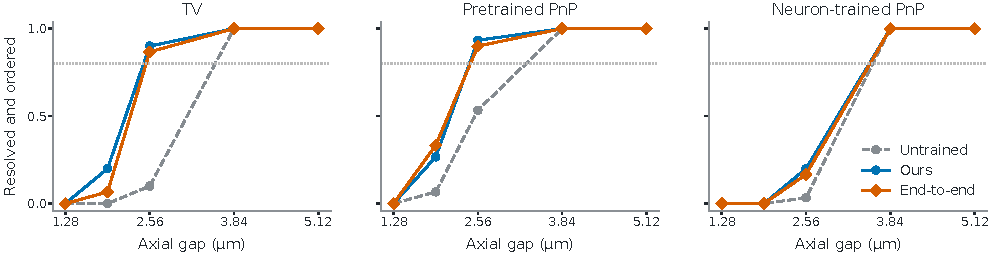
\includegraphics[width=\linewidth]{crossing_curves.pdf}
\caption{Full-dose equal-branch crossing curves for all three iterative methods, at $C=8$ and matched nominal dose. Each point pools three lateral geometries, two axial centers and five draws. The qualifying-gap rule requires at least 80\,\% success at each center separately and at all larger tested gaps. Under neuron-trained PnP, both the untrained and our plates qualify at $3.84\um$. Zero-gap controls have no false splitting.}
\label{fig:s:fullcrossings}
\end{figure*}

\paragraph{Merged neuronal alternatives.}
A reference column is called layered when it belongs to the signal mask and has at least two peaks under the same relative height/prominence rule. For each corresponding fine-grid lateral column, we move its intensity to its axial centroid, distributing mass between the two neighboring planes to preserve that centroid exactly. Other columns remain unchanged. The resulting alternative preserves the fine-grid lateral projection and each modified column's centroid while changing its depth profile. One crop has no eligible columns, leaving 59. These are constructed candidates, not solutions optimized over a measurement-consistency set; concentrated intensities need not remain below the original normalized peak.

For noise-free expected counts $\mu$ of the reference and $\nu(c)$ of a brightness-scaled alternative, we compute
\begin{equation}
D_{\mathrm P}(\mu\Vert\nu)=\sum_i\left[\mu_i\log\frac{\mu_i}{\nu_i}+\nu_i-\mu_i\right].
\end{equation}
The simulator evaluates both objects on the fine grid, using each matched direction subset and the same exposure. Without background, the profiled scale is the ratio of total reference to alternative expected counts. With background, the numerical fit searches a log-scale interval of $[-1,1]$ around the total-signal estimate. Crop scores average five subsets. The geometric mean of the crop-level learned/untrained ratios is 9.99 (95\,\% CI: 8.66--11.79) without background and 10.4 with background. Against the end-to-end plate, our ratio is 2.00 (1.91--2.09), with higher divergence on all 59 eligible crops. The draw-average is taken within each crop before forming the ratios. Untrained-plate divergences can already be large; the ratio is a diagnostic of these specified alternatives, not a probability of successful reconstruction. No KL-to-reconstruction-success guarantee is claimed.

\paragraph{Additional neuronal structure metrics.}
Layered columns carry about 17\,\% of reference signal on average. \Cref{tab:s:layered} uses the completed primary reconstruction rows and the 59 crops with eligible columns; one crop has none. Relative to the untrained plate, our plate lowers their profile W1 by 34\,\% with TV, 42\,\% with pretrained PnP and 28\,\% with neuron-trained PnP. The end-to-end plate has higher W1 than ours under TV, no established difference under either PnP method, and lower W1 with its own decoder. These descriptive subset results contextualize the single-column figures. Most eligible columns contain intensity structure within thick branches, so lower profile error does not establish separation of distinct neuronal branches or a larger benefit than in centroid accuracy.

A prespecified TV comparison did not establish a larger relative profile gain than centroid gain on layered columns: the difference was $-0.7$ percentage points (95\,\% CI: $-2.9$ to $+1.5$). PnP subset statistics remain descriptive because an earlier prespecified PSNR reproduction tolerance of $0.05$\,dB was not met; the completed full-field reruns use the numerical checks documented in \cref{sec:s:evaluation}.

\begin{table*}[t]
\centering\small
\widetab{\begin{tabular}{lrrrll}
\toprule
Reconstruction & Untrained & Ours & End-to-end & Ours vs. untrained & End-to-end minus ours \\
\midrule
TV & 0.467 & 0.309 & 0.318 & $-33.8\%$ [$-36.3$, $-31.7$] & $+0.009$ [$+0.004$, $+0.015$] \\
Pretrained PnP & 0.641 & 0.369 & 0.370 & $-42.4\%$ [$-46.5$, $-38.5$] & $+0.001$ [$-0.008$, $+0.009$] \\
Neuron-trained PnP & 0.374 & 0.271 & 0.272 & $-27.6\%$ [$-28.8$, $-26.4$] & $+0.001$ [$-0.002$, $+0.004$] \\
Feed-forward & 0.518 & 0.387 & 0.352 & $-25.4\%$ [$-29.6$, $-21.8$] & $-0.035$ [$-0.045$, $-0.028$] \\
\bottomrule
\end{tabular}
}
\caption{Profile W1 on layered reference columns: 59 eligible crops, $C=8$, five draws per crop, using the same completed reconstructions as the primary table. Errors and absolute end-to-end-minus-ours differences are in $\mu$m; brackets are paired cell-bootstrap 95\,\% intervals. Feed-forward decoders have the training histories in \cref{sec:s:joint}.}
\label{tab:s:layered}
\end{table*}

On all 60 crops, we also report centerline Dice \cite{shit2021}, which compares a reference mask at 10\,\% of peak intensity with an estimated mask retaining the same number of voxels, followed by 3D skeletonization. Scores rise from 0.79 to 0.84 for TV, 0.75 to 0.84 for pretrained PnP and 0.85 to 0.88 for neuron-trained PnP. This thresholded metric is depth-sensitive but does not substitute for branch tracing or connectivity validation.

\section{Measurement, photon and alignment controls}
\label{sec:s:budgets}

\paragraph{Dose convention.}
Each encoder's excitation is divided by its mean over the specimen analysis grid and the full 256-direction scan. This fixes the deposited excitation per complete scan. For $k$ directions, exposure is multiplied by $256/k$. Random subsets therefore match nominal dose in expectation, not exactly for each subset. The per-specimen exposure is set from the random plate's full-scan mean signal and reused for every encoder. Equal deposited dose does not force identical detected counts: illumination can correlate differently with the specimen. For the two learned plates, mean detected signal changes by about $-1$ to $-2$\,\% across the 12 crops, with individual changes approximately $-12$ to $+9$\,\%.

\paragraph{Measurement compression.}
\Cref{tab:s:compression} reports both depth metrics at $C=1,4,8$. These values count all camera samples, not camera images alone. At matched nominal dose, fewer directions mean longer exposure per image. The learned 32-image acquisition gives lower W1 than the 256-image random acquisition for TV and pretrained PnP, but the close neuron-trained-PnP means do not establish equivalence. The TV curve is not monotone in compression: validation can prefer a stronger regularization weight at $C=4$, which smooths neuronal features more than at $C=8$.

\begin{table*}[t]
\centering\small
\widetab{\begin{tabular}{@{}llcccccc@{}}
\toprule
Reconstruction & Plate & W1, $C=1$ & Centroid & W1, $C=4$ & Centroid & W1, $C=8$ & Centroid\\
\midrule
TV & Random & 0.249 & 0.187 & 0.298 & 0.223 & 0.318 & 0.243\\
TV & Learned, seed 0 & 0.170 & 0.135 & 0.208 & 0.166 & 0.196 & 0.153\\
TV & Learned, seed 1 & 0.160 & 0.124 & 0.202 & 0.158 & 0.195 & 0.151\\
Pretrained PnP & Random & 0.413 & 0.357 & 0.445 & 0.384 & 0.496 & 0.431\\
Pretrained PnP & Learned, seed 0 & 0.222 & 0.184 & 0.254 & 0.212 & 0.277 & 0.231\\
Pretrained PnP & Learned, seed 1 & 0.213 & 0.173 & 0.249 & 0.206 & 0.279 & 0.234\\
Neuron-trained PnP & Random & 0.203 & 0.161 & 0.234 & 0.184 & 0.282 & 0.221\\
Neuron-trained PnP & Learned, seed 0 & 0.142 & 0.110 & 0.167 & 0.130 & 0.206 & 0.163\\
\bottomrule
\end{tabular}
}
\caption{Measurement budgets on the 12 prespecified crops. W1 and centroid errors are in $\mu$m and come from the same reconstruction rows. $C=1$ uses all 256 directions; $C=4,8$ average five subsets of 64 and 32 directions. No missing independent-initialization results are imputed.}
\label{tab:s:compression}
\end{table*}

\paragraph{Noise conditions.}
The nominal model uses Poisson shot noise. The background condition adds a uniform mean equal to the random plate's mean expected signal for the same exposure, plus independent Gaussian read noise with standard deviation 2 electrons. The known mean background is subtracted before reconstruction. The same background level, exposure and noise protocol are used for each encoder. A separate low-dose condition reduces exposure to one tenth. Scalar reconstruction parameters are revalidated for each changed noise condition, while networks stay fixed. \Cref{tab:s:noise} reports all three methods.

\begin{table*}[t]
\centering\small
\widetab{\begin{tabular}{@{}llcccccc@{}}
\toprule
Condition & Reconstruction & W1, random & W1, learned & Centroid, random & Centroid, learned & W1 change & Centroid change\\
\midrule
Shot noise & TV & 0.318 & 0.196 & 0.243 & 0.153 & $-38$\,\% [$-43$, $-34$] & $-37$\,\% [$-41$, $-34$]\\
Shot noise & Pretrained PnP & 0.496 & 0.277 & 0.431 & 0.231 & $-44$\,\% [$-50$, $-39$] & $-46$\,\% [$-53$, $-41$]\\
Shot noise & Neuron-trained PnP & 0.282 & 0.206 & 0.221 & 0.163 & $-27$\,\% [$-34$, $-20$] & $-26$\,\% [$-35$, $-18$]\\
Background + read noise & TV & 0.324 & 0.227 & 0.249 & 0.180 & $-30$\,\% [$-38$, $-22$] & $-28$\,\% [$-36$, $-20$]\\
Background + read noise & Pretrained PnP & 0.627 & 0.297 & 0.548 & 0.247 & $-53$\,\% [$-57$, $-48$] & $-55$\,\% [$-60$, $-50$]\\
Background + read noise & Neuron-trained PnP & 0.288 & 0.210 & 0.228 & 0.166 & $-27$\,\% [$-35$, $-19$] & $-27$\,\% [$-36$, $-18$]\\
0.1 dose & TV & 0.466 & 0.292 & 0.365 & 0.236 & $-37$\,\% [$-45$, $-29$] & $-35$\,\% [$-44$, $-28$]\\
0.1 dose & Pretrained PnP & 0.834 & 0.407 & 0.733 & 0.352 & $-51$\,\% [$-57$, $-45$] & $-52$\,\% [$-58$, $-45$]\\
0.1 dose & Neuron-trained PnP & 0.345 & 0.239 & 0.269 & 0.186 & $-31$\,\% [$-37$, $-24$] & $-31$\,\% [$-38$, $-24$]\\
\bottomrule
\end{tabular}
}
\caption{Noise controls on 12 crops at $C=8$. Errors are in $\mu$m; changes and cell-bootstrap 95\,\% intervals compare the learned and random plates within the same condition.}
\label{tab:s:noise}
\end{table*}

\paragraph{Photon budget.}
The dose sweep uses factors $0.1$, $0.3$, $1$ and $3$ of the nominal exposure (\cref{tab:s:dose}). At dose $0.3$, learned-plate W1 is $0.234$, $0.302$ and $0.220\um$ for TV, pretrained PnP and neuron-trained PnP, compared with $0.318$, $0.496$ and $0.282\um$ for the random plate at dose 1. These reductions of 26\,\%, 39\,\% and 22\,\% describe the tested simulation and inference budgets. The random curve's flattening between doses 1 and 3 is not evidence of a fundamental photon limit.

\begin{table*}[t]
\centering\small
\begin{tabular}{@{}lccccc@{}}
\toprule
Reconstruction & Nominal dose & W1, random & W1, learned & Centroid, random & Centroid, learned\\
\midrule
TV & 0.1 & 0.466 & 0.292 & 0.365 & 0.236\\
TV & 0.3 & 0.442 & 0.234 & 0.341 & 0.185\\
TV & 1 & 0.318 & 0.196 & 0.243 & 0.153\\
TV & 3 & 0.315 & 0.192 & 0.242 & 0.151\\
Pretrained PnP & 0.1 & 0.834 & 0.407 & 0.733 & 0.352\\
Pretrained PnP & 0.3 & 0.631 & 0.302 & 0.550 & 0.251\\
Pretrained PnP & 1 & 0.496 & 0.277 & 0.431 & 0.230\\
Pretrained PnP & 3 & 0.494 & 0.276 & 0.430 & 0.230\\
Neuron-trained PnP & 0.1 & 0.345 & 0.239 & 0.269 & 0.186\\
Neuron-trained PnP & 0.3 & 0.304 & 0.220 & 0.236 & 0.174\\
Neuron-trained PnP & 1 & 0.282 & 0.207 & 0.221 & 0.164\\
Neuron-trained PnP & 3 & 0.275 & 0.203 & 0.218 & 0.162\\
\bottomrule
\end{tabular}

\caption{Dose sweep at $C=8$, 12 crops. W1 and centroid errors ($\mu$m) are computed from the same reconstructions. Each exposure factor is relative to the matched nominal-dose protocol.}
\label{tab:s:dose}
\end{table*}

\paragraph{Alignment.}
Distance perturbations set $D=6.1$ or $7.1\um$. In the characterized case, the operator is rebuilt from the known distance and scalar reconstruction parameters are revalidated; the phase is unchanged. In the nominal-operator case, reconstruction ignores the perturbation. Lateral error shifts the plate by one $0.32\um$ feature. Pointing errors are offsets of 0.005 or 0.01 in transverse direction cosine. All comparisons use neuron-trained PnP, $C=8$, the same 12 crops and five draws.

\Cref{tab:s:alignment} separates these assumptions. Known distance changes retain the optical gain. Ignoring distance or lateral registration can make the learned plate worse than the random one, including an 11\,\% W1 increase for a one-feature lateral shift. Rebuilding an operator with a known perturbation is not an experimentally demonstrated calibration procedure. Phase-quantization experiments are not used to claim a fabricable low-level plate: the simulated surround was not quantized with the trained center.

\begin{table*}[t]
\centering\small
\widetab{\begin{tabular}{@{}lcccccc@{}}
\toprule
Condition & W1, random & W1, learned & Centroid, random & Centroid, learned & W1 change & Centroid change\\
\midrule
none (design) & 0.282 & 0.206 & 0.221 & 0.163 & $-27$\,\% [$-34$, $-20$] & $-26$\,\% [$-35$, $-18$]\\
Known: D=6.1 & 0.285 & 0.205 & 0.225 & 0.162 & $-28$\,\% [$-35$, $-22$] & $-28$\,\% [$-37$, $-20$]\\
Known: D=7.1 & 0.284 & 0.209 & 0.226 & 0.166 & $-27$\,\% [$-34$, $-20$] & $-26$\,\% [$-35$, $-19$]\\
Nominal operator: scan tilt 0.005 & 0.318 & 0.254 & 0.253 & 0.196 & $-20$\,\% [$-25$, $-16$] & $-22$\,\% [$-30$, $-15$]\\
Nominal operator: scan tilt 0.01 & 0.379 & 0.328 & 0.308 & 0.251 & $-13$\,\% [$-16$, $-10$] & $-18$\,\% [$-22$, $-15$]\\
Nominal operator: D=6.1 & 0.563 & 0.586 & 0.528 & 0.571 & $+4$\,\% [$+0.3$, $+8$] & $+8$\,\% [$+3$, $+14$]\\
Nominal operator: D=7.1 & 0.447 & 0.473 & 0.383 & 0.438 & $+6$\,\% [$+5$, $+7$] & $+14$\,\% [$+12$, $+17$]\\
Nominal operator: lateral shift 1 feature & 0.451 & 0.500 & 0.372 & 0.400 & $+11$\,\% [$+2$, $+23$] & $+7$\,\% [$-0.4$, $+19$]\\
\bottomrule
\end{tabular}
}
\caption{Alignment controls with neuron-trained PnP. Errors are in $\mu$m; changes compare learned and random plates under the same perturbation. ``Known'' means the offset is supplied to operator assembly and validation; ``nominal operator'' means it is ignored. Positive changes favor the random plate.}
\label{tab:s:alignment}
\end{table*}

\section{Complementary uncertainty analyses}
\label{sec:s:uncertainty}

These analyses ask different questions from the main reconstruction tests. Centroid intervals quantify an empirical depth error rate after reconstruction. Set-membership bounds assess admissible voxel intensities without a learned prior. Neither supplies a connectivity guarantee for the neuronal reconstructions.

\paragraph{Conformal centroid intervals.}
We form $\hat z_c\pm\lambda$ around each reconstructed axial centroid. For a volume, $L(\lambda)$ is the reference-signal-weighted fraction of evaluated columns whose true centroid lies outside the interval. It is bounded by one and decreases with $\lambda$. Conformal risk control \cite{angelopoulos2024crc} selects
\begin{equation}
\hat\lambda=\inf\left\{\lambda:\frac{n}{n+1}\hat R_n(\lambda)+\frac1{n+1}\le\alpha\right\},
\end{equation}
where $\hat R_n$ averages the loss over $n$ calibration volumes. Under exchangeability of the calibration volumes and a new volume, $\mathbb E[L(\hat\lambda)]\le\alpha$. This controls expected signal-weighted miscoverage, not each column's or specimen's coverage.

We use neuron-trained PnP at $C=8$, target $\alpha=0.1$ and encoder-specific calibration on 35 non-overlapping crops from a held-out SOM009 stack. A 240-crop overlapping set is a sensitivity analysis, not independent replication. On the 12 prespecified test crops, the learned seed-0 half-width decreases from $0.646$ to $0.474\um$ (26.7\,\%), with empirical miscoverage 0.075 versus 0.060 for the untrained plate (\cref{tab:s:conformal}). The test animals differ from the calibration animal, so exchangeability is not established; observed miscoverage is empirical rather than a cross-animal guarantee.

\begin{table}[t]
\centering\small
\coltab{\begin{tabular}{@{}l cc cc@{}}\toprule
 & \multicolumn{2}{c}{35 non-overlapping crops} & \multicolumn{2}{c}{all 240 crops}\\
\cmidrule(lr){2-3}\cmidrule(l){4-5}
plate & $\hat\lambda$ ($\mu$m) & test miscov. & $\hat\lambda$ ($\mu$m) & test miscov.\\\midrule
random & 0.646 & 0.060 & 0.570 & 0.085\\
learned, seed 0 & 0.474 & 0.075 & 0.422 & 0.091\\
learned, seed 1 & 0.486 & 0.060 & 0.422 & 0.081\\
\bottomrule\end{tabular}
}
\caption{Calibrated centroid half-widths and empirical signal-weighted test miscoverage. The 240-crop analysis reuses overlapping regions. Seed 1 gives $0.486\um$ on the primary 35-crop calibration set.}
\label{tab:s:conformal}
\end{table}

\paragraph{Voxel bounds without a learned prior.}
Given $\bx\in[0,1]^N$, define
\begin{equation}
\mathcal C(\by)=\{\bx:\ \ell_i\le(\bA\bx)_i\le h_i,\ 0\le\bx\le1\}.
\end{equation}
For a nonempty set, minimizing and maximizing $x_j$ gives the smallest and largest voxel intensities compatible with the stated constraints \cite{milanese1991,haldar2023}. We solve these linear programs with HiGHS \cite{huangfu2018}. The reconstruction's quadratic data term does not automatically place its output in this set.

The reduced field contains $4\times12\times12$ reconstruction voxels and $3\times3$ camera samples per image, using 32 fixed directions. Thus, $N=576$ and $M=288$; this is a separate geometry, not the full-field $C=8$ experiment. Plates are trained separately on this reduced geometry; no reflected-depth pair qualifies for the full-grid weighting rule, so all off-diagonal weights are one.

The ancillary Gaussian model uses reference full-scan mean $m_p$ for the untrained plate and mean $m_e$ for an encoder, with $\sigma_e=m_p10^{-q/10}\sqrt{k/256}\sqrt{m_e/m_p}$ and reference parameter $q=15$. At $q=15$, this is a spatially uniform Gaussian approximation to the main photon model at each encoder's mean signal, rather than a pixelwise Poisson variance. The formula defines $q$ explicitly; it is not a standard RMS SNR. Intervals use $y_i\pm z\sigma_e$, where $z=\Phi^{-1}(1-0.05/(2\cdot2880))$. The family contains all 2304 rows of the 256-direction reduced scan plus up to 576 projection constraints. Using the same correction for every subset gives at least 95\,\% simultaneous coverage under the stated Gaussian model and exact reduced linear operator. Unmodeled optical or specimen discretization error would require a separate allowance.

Across 24 synthetic phantoms and three noise realizations each, the learned reduced-field plates narrow mean voxelwise bound width by about 21\,\%. On 48 neuronal windows, however, bounds span the full admissible range for every voxel at the tested settings. Better neuronal reconstruction in the main study therefore does not imply unique voxel intensities or uniquely identified connections. These negative neuronal results are retained as limits of the measurement-only analysis, not as optical-learning performance measures.

\section{Neuronal views and display selection}
\label{sec:s:views}

\paragraph{Illustrative unequal-peak example.}
The main neuronal figure uses SOM006\_cell3\_c0 with pretrained PnP at $C=8$ and nominal dose. We screened the 60 references for interior columns with exactly two peaks, separated by at least three planes, and a weaker-to-stronger height ratio of 0.2--0.6. Peaks must meet the height and prominence thresholds used for layered-column evaluation. A supported region contains the center and at least four neighboring eligible columns with corresponding peak planes within one plane. This gives 685 eligible columns and 13 supported regions in six crops. An expanded screen with two supporting neighbors was also examined; the selected column meets the original, stricter rule. We inspected paired reconstruction outcomes and selected the displayed column for its lower W1 and better retention of the weaker component across all five subsets. This is an outcome-selected local illustration, not a representative or aggregate comparison.

The column is $(x,y)=(35,30)$, with reference peaks at planes 3 and 11 (zero-based) and a weaker-to-stronger height ratio of 0.59. The axial band spans rows 34--36. \Cref{tab:s:unequalpeaks,fig:s:unequalpeaks} give the five-subset errors and profiles, including raw intensity. Our column W1 is lower than both controls in every subset. Among the 13 original region centers, our and end-to-end W1 beat the untrained plate in all five subsets at 10 and 8 centers, respectively; each learned plate beats both others at one center. The larger region around the displayed column does not share its ordering: our and end-to-end mean W1 are $0.223$ and $0.210\um$ over its five columns, and $0.220$ and $0.218\um$ over the crop. The displayed volumes reproduce the recorded rows within $0.002$\,dB PSNR and $0.0003\um$ crop W1.

\begin{table}[t]
\centering\small
\begin{tabular}{lrrr}
\toprule
Subset & Untrained & Ours & End-to-end \\
\midrule
1 & 0.344 & 0.117 & 0.231 \\
2 & 0.514 & 0.110 & 0.366 \\
3 & 0.490 & 0.102 & 0.147 \\
4 & 0.648 & 0.150 & 0.296 \\
5 & 0.815 & 0.169 & 0.346 \\
\midrule
Mean & 0.562 & \textbf{0.130} & 0.277 \\
\bottomrule
\end{tabular}
\caption{Column W1 ($\mu$m) for the selected unequal-peak example across the five recorded direction subsets. Subset 1 is displayed in the main figure.}
\label{tab:s:unequalpeaks}
\end{table}

\begin{figure*}[t]
\centering
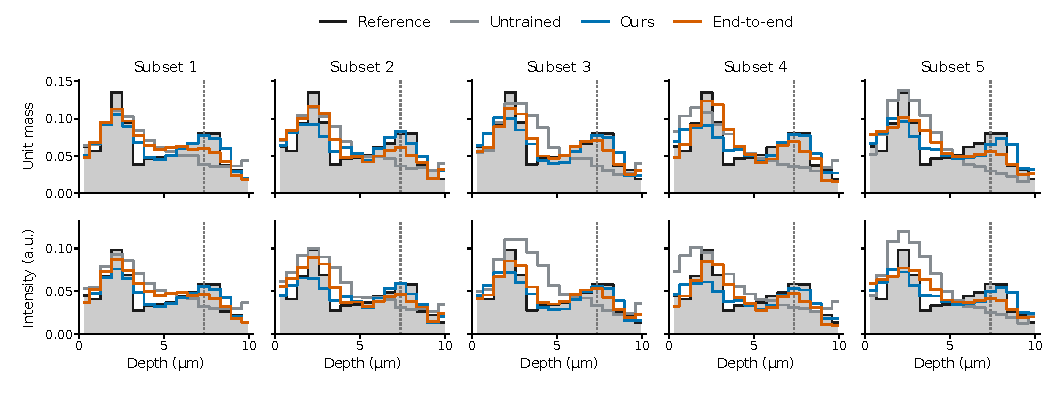
\includegraphics[width=\linewidth]{unequal_peak_profiles.pdf}
\caption{The selected main-figure column across all five direction subsets. Top: unit-mass axial profiles used for column W1. Bottom: raw intensities on one shared linear scale. Gray fills show the reference, and the dashed line marks its weaker peak. Our plate preserves this component's relative strength more closely across subsets; in Subset 1, it also underestimates the stronger peak most.}
\label{fig:s:unequalpeaks}
\end{figure*}

\paragraph{Reference-only selection.}
Before opening reconstructions for figure selection, we computed reference features for all 60 crops. Eligible crops had at least 10 skeleton endpoints (the upper quartile) and a 10--90\,\% column-centroid range of at least $3.64\um$ (the median), indicating several branches and substantial depth extent. Eight crops qualified. We ranked them by reference signal in columns with at least two axial peaks. The first was SOM004\_cell2\_x7; the companion was the highest-ranked eligible crop from another animal, SOM006\_cell1\_x7.

After selection, their W1-gain ranks among 60 crops were 52/45/23 and 45/46/43 for TV/pretrained/neuron-trained PnP, where rank 1 is the largest reduction. These are typical-to-lower-gain examples. We retain both alongside the main figure's unequal-peak illustration. \Cref{fig:s:mainviews,fig:s:companion} show all three iterative methods for these crops. The full-cell panels supply two-photon context; only the marked crops generate simulated measurements.

\paragraph{Views and scales.}
For the two reference-selected crops, the axial band maximizes reference signal in layered columns over three consecutive lateral rows ($1.92\um$). Within it, the profile column has the largest reference signal among layered columns whose two highest peaks are at least three planes apart. This gives $(x,y)=(35,44)$ in the first crop and $(42,16)$ in the companion; the first lies three voxels from an edge and was retained unchanged. Their displayed volumes use noise draw 0. These columns favor the end-to-end plate more strongly than the crop-wide error; they illustrate local behavior, not a population ranking.

Depth-colored projections tint each plane with an approximately constant-lightness depth color at its linear intensity, then take the maximum independently in each color channel. Overlapping layers may mix colors or be dominated by the brighter layer, so axial bands, profiles and W1 maps accompany the projections. Fluorescence intensity images---bands, slabs, reference projections and two-photon contexts---use inverted gray, so darker pixels carry more signal. Reconstruction panels use one linear range per crop, from zero to the 99.5th percentile of its reference maximum projection, with no gamma, smoothing or per-panel rescaling. W1 maps use a shared 0--$1\um$ scale from light pink at zero to deep purple at or above $1\um$; white marks unscored pixels outside the reference signal mask. Rows and columns correspond to $x$ and $y$ throughout; axial depth increases downward.

Full-cell contexts are maximum projections of the original two-photon stacks, linearly clipped at their 99.8th percentile. They retain tissue coordinates ($0.25\um$ lateral sampling), whereas reconstructed views use simulation coordinates. The boxed $32\times32\times32\um^3$ tissue crops become $30.72\times30.72\times10.24\um^3$ simulated volumes. The reference-selected reconstructions reproduce the recorded rows within $0.018$\,dB PSNR and $0.001\um$ W1. The following full views retain context and individual profiles.

\begin{figure*}[t]
\centering
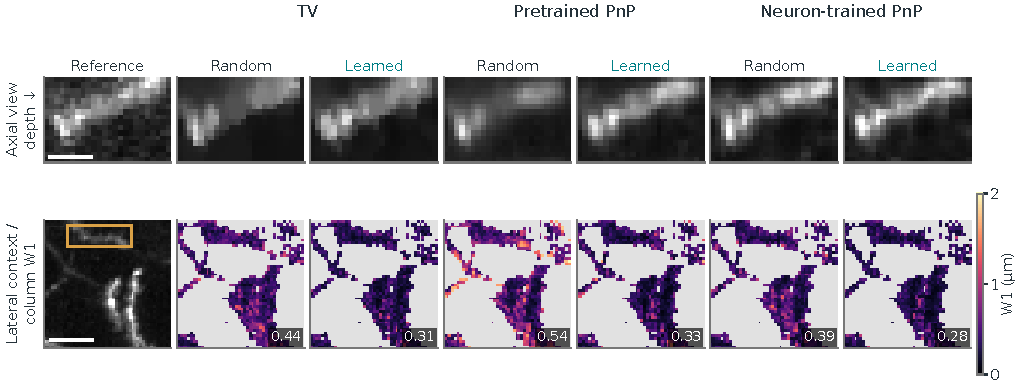
\includegraphics[width=\linewidth]{neuron_comparison.pdf}
\caption{All three iterative methods for the first reference-selected crop. Left: matched axial bands for the reference, untrained, our and end-to-end plates. Right: column-W1 maps with draw-0 crop means below. White marks pixels outside the reference signal mask. The $5\um$ bar applies to both axes of each band; maps span the full $30.72\um$ lateral field.}
\label{fig:s:mainviews}
\end{figure*}

\begin{figure*}[t]
\centering
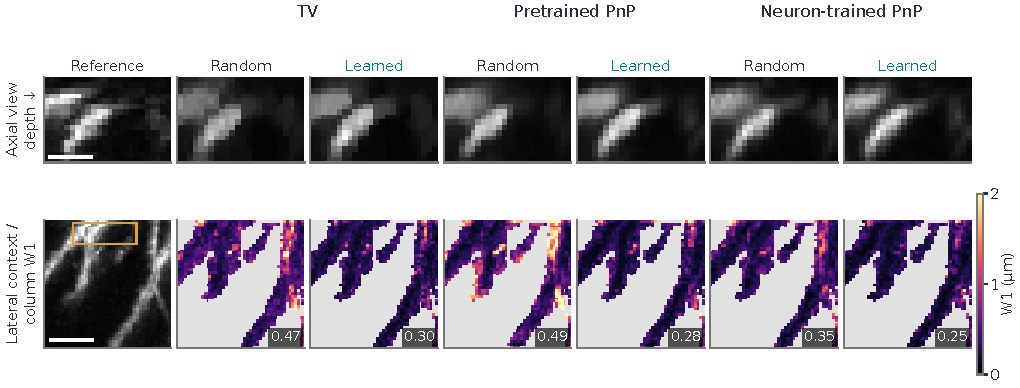
\includegraphics[width=\linewidth]{neuron_companion.pdf}
\caption{The companion crop from another animal, using the same band and error-map conventions as \cref{fig:s:mainviews}. Values are draw-0 crop W1 in $\mu$m; the bar is $5\um$.}
\label{fig:s:companion}
\end{figure*}

\begin{figure*}[t]
\centering
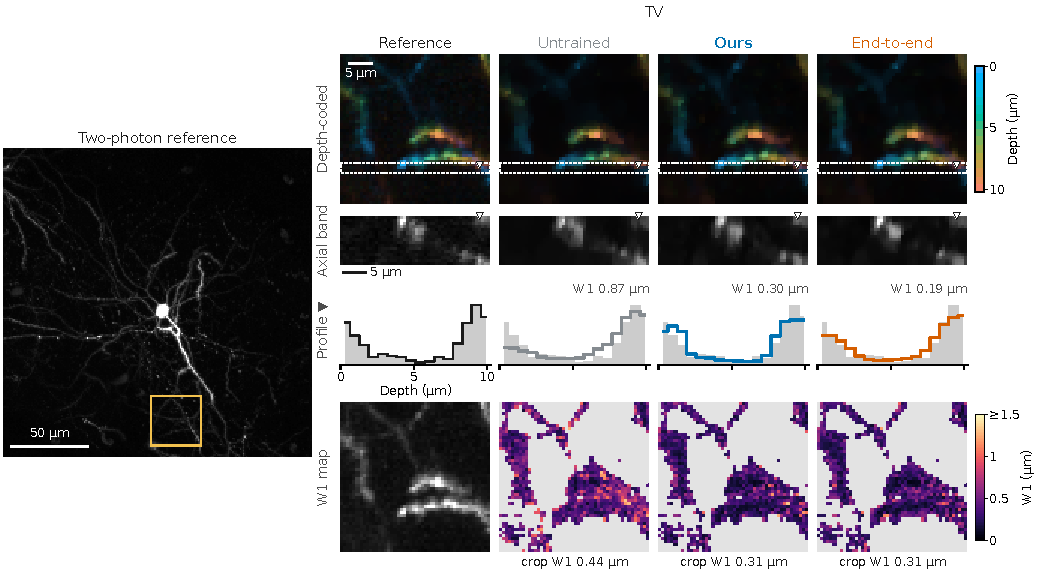
\includegraphics[width=\linewidth]{neuron_tv.pdf}
\caption{First crop with TV. Context, projection, band, profile and error-map conventions match the main neuronal figure. The marked profile is one reference-selected column; the means below the maps summarize all reference-signal columns for this draw.}
\label{fig:s:tvview}
\end{figure*}

\begin{figure*}[t]
\centering
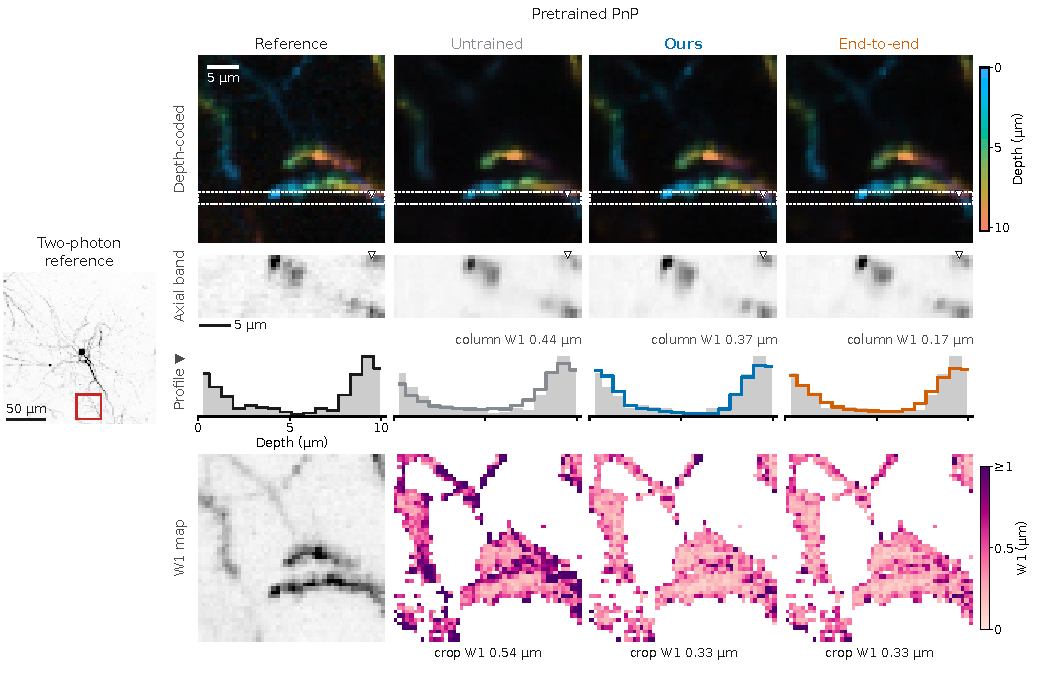
\includegraphics[width=\linewidth]{neuron_pretrained.pdf}
\caption{First reference-selected crop with pretrained PnP, retained from the earlier main figure. The marked column favors end-to-end more strongly than the crop mean.}
\label{fig:s:pretrainedview}
\end{figure*}

\begin{figure*}[t]
\centering
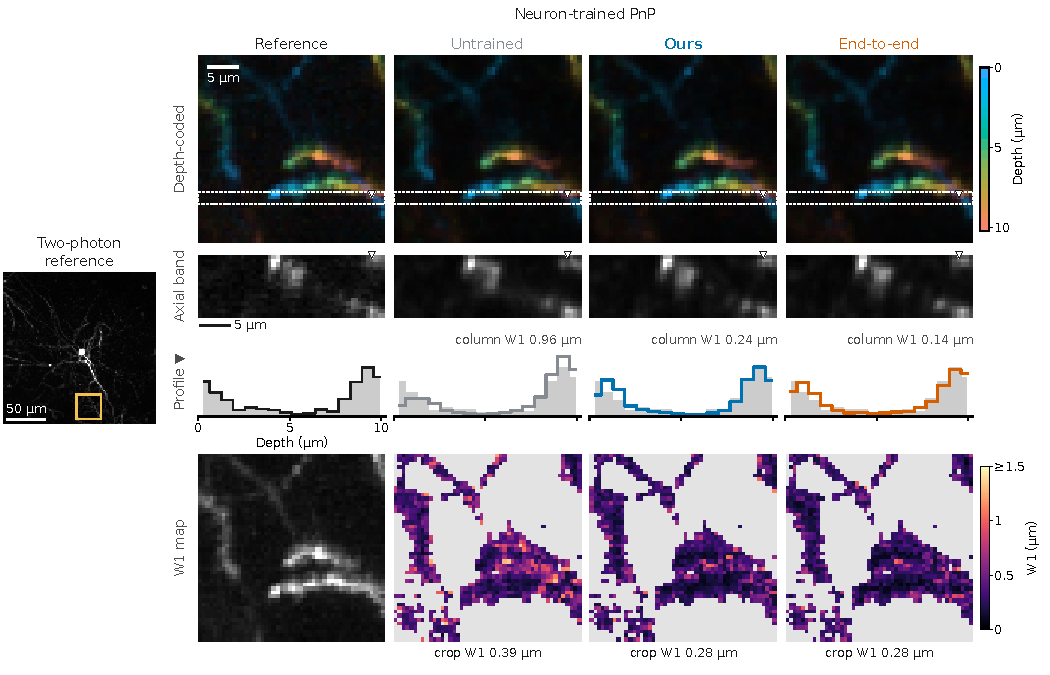
\includegraphics[width=\linewidth]{neuron_trained.pdf}
\caption{First crop with neuron-trained PnP. Context, projection, band, profile and error-map conventions match the main neuronal figure. The marked profile is one reference-selected column; the means below the maps summarize all reference-signal columns for this draw.}
\label{fig:s:neuronview}
\end{figure*}

\begin{figure*}[t]
\centering
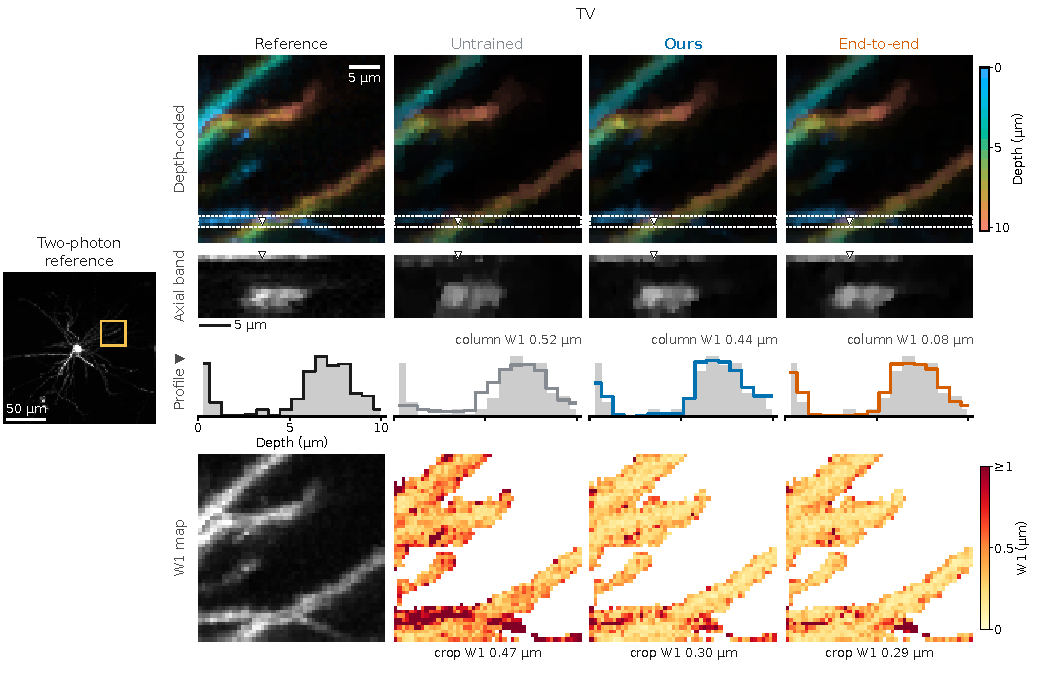
\includegraphics[width=\linewidth]{companion_tv.pdf}
\caption{Companion crop with TV. Context, projection, band, profile and error-map conventions match the main neuronal figure. The marked profile is one reference-selected column; the means below the maps summarize all reference-signal columns for this draw.}
\label{fig:s:companTV}
\end{figure*}

\begin{figure*}[t]
\centering
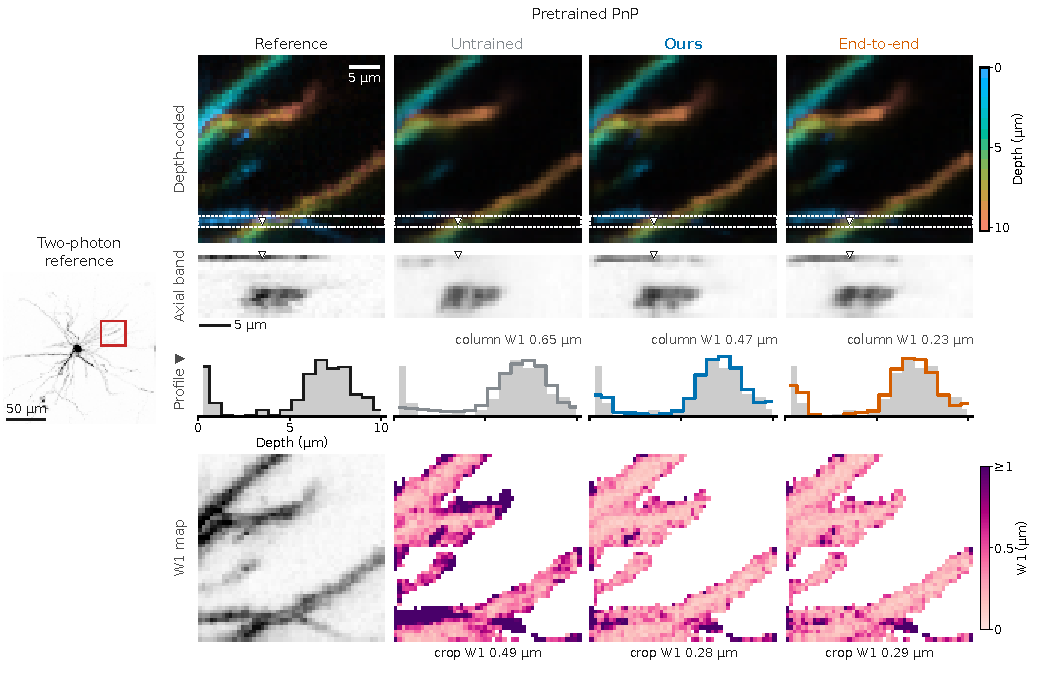
\includegraphics[width=\linewidth]{companion_pretrained.pdf}
\caption{Companion crop with pretrained PnP. Context, projection, band, profile and error-map conventions match the main neuronal figure. The marked profile is one reference-selected column; the means below the maps summarize all reference-signal columns for this draw.}
\label{fig:s:companPre}
\end{figure*}

\begin{figure*}[t]
\centering
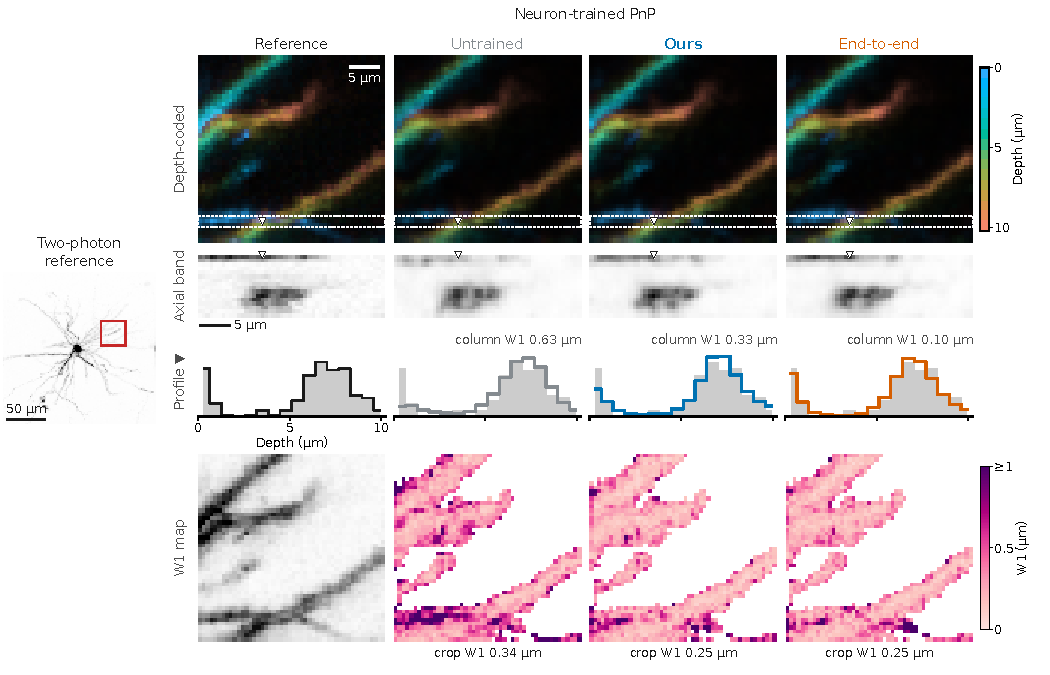
\includegraphics[width=\linewidth]{companion_trained.pdf}
\caption{Companion crop with neuron-trained PnP. Context, projection, band, profile and error-map conventions match the main neuronal figure. The marked profile is one reference-selected column; the means below the maps summarize all reference-signal columns for this draw.}
\label{fig:s:companNeur}
\end{figure*}

\begin{figure*}[t]
\centering
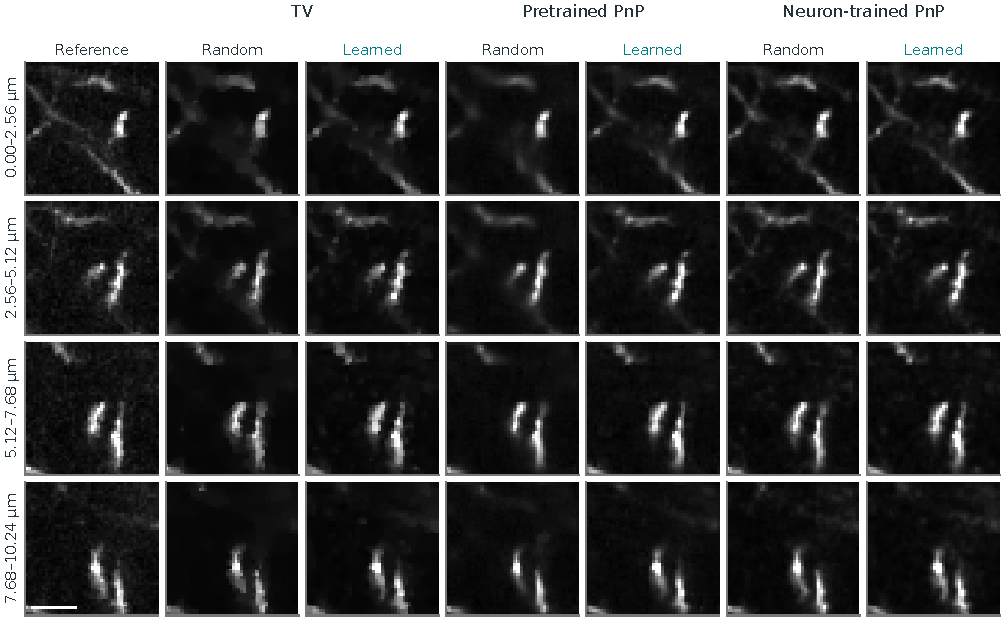
\includegraphics[width=\linewidth]{neuron_slabs_a.pdf}
\caption{Depth slabs of the first neuronal example, with maximum projections over four consecutive depth planes ($2.56\um$ per slab). Reference and all reconstructions share the same linear intensity range across slabs. Slab views expose signal spread into depths absent from the corresponding reference slab. These are qualitative placement comparisons, not branch-separation measurements. Bar: $10\um$.}
\label{fig:s:slabsa}
\end{figure*}

\begin{figure*}[t]
\centering
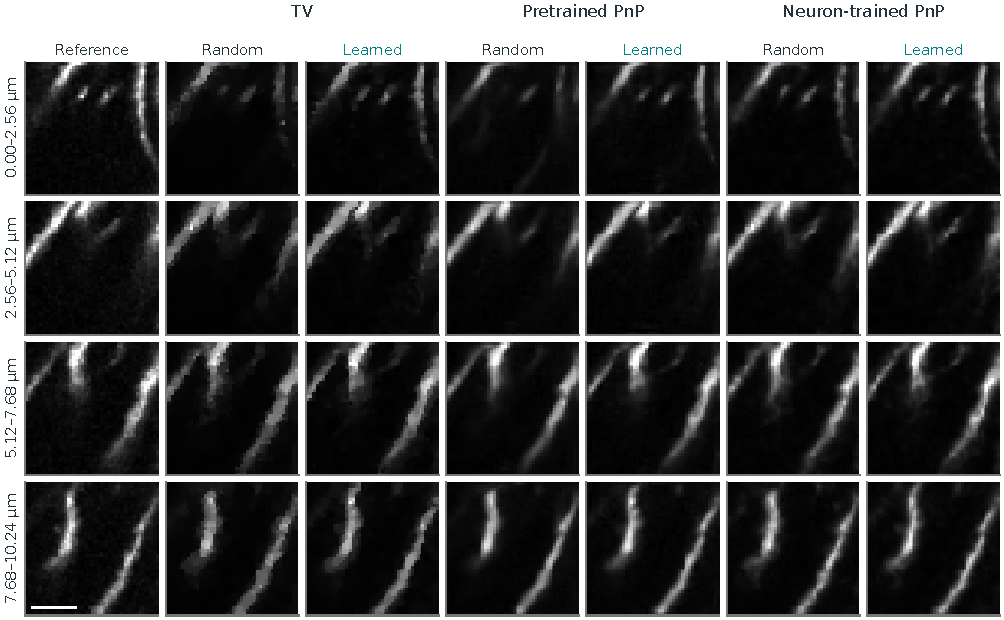
\includegraphics[width=\linewidth]{neuron_slabs_b.pdf}
\caption{The companion crop from another animal, with the same depth-slab conventions. Stronger priors reduce diffuse signal for both plates; the optical difference is smaller under neuron-trained PnP. The full views retain features missed by either encoder.}
\label{fig:s:slabsb}
\end{figure*}

\paragraph{A feature missed by both plates.}
A separate weak-feature illustration uses the earlier reference-selected companion band: the layered column with largest reference mass whose two highest peaks are at least three planes apart. Its selected column, $(x,y)=(18,3)$, contains a weak shallow peak at plane 2 above a deeper peak at plane 9. The shallow peak is 24.5\,\% of the column maximum and carries 7.8\,\% of its signal in planes 1--3. None of the six untrained- and our-plate reconstructions has a matched shallow peak; that signal becomes a low plateau (\cref{fig:s:weakprofile}). This limit coexists with lower average W1 and improved placement of brighter features.

\begin{figure*}[t]
\centering
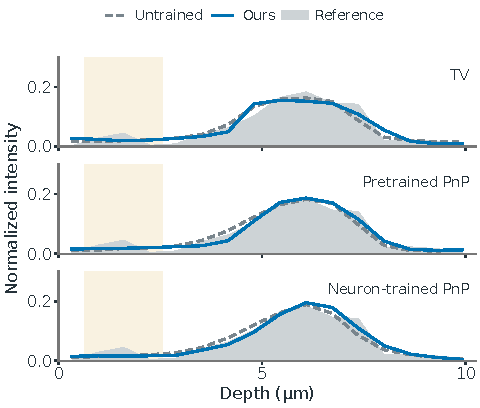
\includegraphics[width=.48\linewidth]{neuron_weak_profile.pdf}
\caption{Reference-selected weak-feature column in the companion crop. Profiles are normalized to unit mass. Both plates miss the shallow reference peak under all three priors, despite the lower average W1 of our plate. This column was fixed from reference structure before inspecting reconstructions.}
\label{fig:s:weakprofile}
\end{figure*}


\onecolumn
\twocolumn
\raggedbottom
{\small
\bibliographystyle{settings/ieeenat_fullname}
\bibliography{references}}
